%--------------------------------------
% Create title frame
\titleframe

%--------------------------------------
% Table of contents
\begin{frame}{Overview}
  \setbeamertemplate{section in toc}[sections numbered]
  \tableofcontents[hideallsubsections]
\end{frame}

\begin{frame} {Lecture overview}
\begin{itemize}
\item The goal of this lecture is to introduce the concept of mathematical programming, particularly linear programming.
\item We also quickly review solution methods for these problems.
\item These tools can then be used for optimal power flow, real-time dispatch, operational planning, or sizing of a microgrid, for instance.
\end{itemize}

 A part of this lecture is based on slides from Pr. Quentin Louveaux at University of Liège.

\end{frame}


\section{Mathematical programming}
\begin{frame} \frametitle{Mathematical programming}
Mathematical programming is a field of applied mathematics that deals with solving optimization problems. 

\vfill

More precisely, it provides a framework and solution methods for computing the \alert{decisions} of an optimization problem, given an \alert{objective function} to minimize or maximize, and (optionally) \alert{constraints} on the decision variables.

\vfill 
Mathematical programming relies on a model of the problem to solve.

\vfill

There is a great variety of mathematical programming problem types, depending on the characteristics of the objective function and constraints and of the restrictions that apply to variables.
	
\end{frame}

\begin{frame} \frametitle{Categories of mathematical programs}
\centering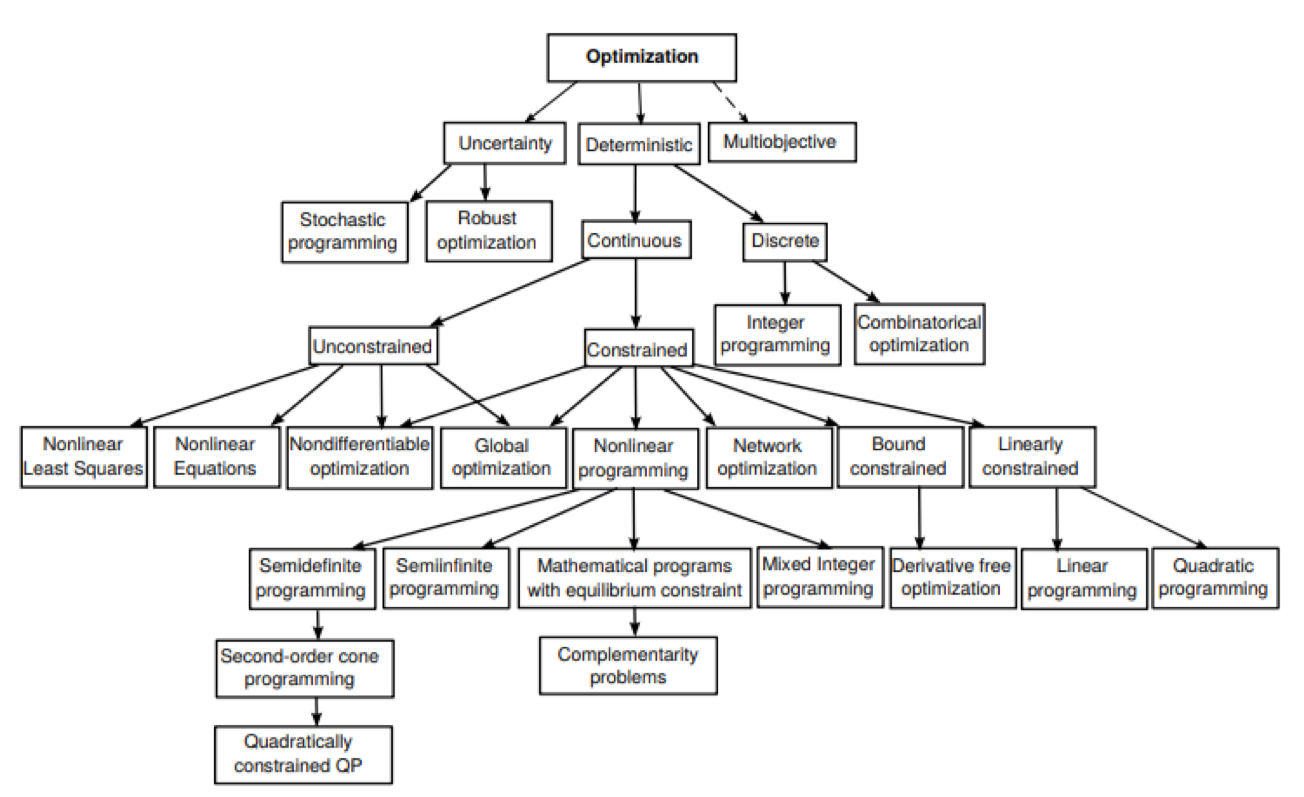
\includegraphics[width=0.7\textwidth]{categories.png}\\
\url{https://neos-guide.org/content/optimization-taxonomy}
\end{frame}

\begin{frame} \frametitle{Categories of mathematical programs}
\scriptsize
\begin{columns}
	\column{5cm}
	\begin{block}{\footnotesize General mathematical program}
		A general mathematical program can be stated as follows:
		\begin{align*}
			\min \; & f(x) \\
			s.t. \; & g(x) \leq 0 \\
			& Ax = 0 \\
			&x \in X
		\end{align*}
		It is very hard to solve, especially when
		\begin{itemize}
		\item objective and constraints are non-linear or even worse non-convex
		\item variables are discrete
		\end{itemize}
	\end{block}
	\column{8cm}
	\begin{block}{\footnotesize Linear program}
            \vspace{-1\baselineskip}
		\begin{align*}
		\min \; & c^Tx \\
		s.t. \; & Ax = b \\
		&x \in \mathbb{R}^n_+
		\end{align*}
		Easy to solve even for large problems.
	\end{block}
	\begin{block}{\footnotesize Mixed-Integer Linear program}
            \vspace{-1\baselineskip}
            \begin{align*}
		\min \; & c^Tx \\
		s.t. \; & Ax = b \\
		&x \in \mathbb{R}^{n_1}_+*\mathbb{Z}^{n_2}_+
		\end{align*}
		Hard problem, but feasible for moderately sized instances.
	\end{block}
\end{columns}
\end{frame}

\section{Linear programming}

\begin{frame}[allowframebreaks]{Linear programming}
	If the objective is \alert{linear} and the constraints are \alert{linear},
	we talk about \alert{linear programming} (LP) or \alert{linear optimization}.
	\begin{block}{LP in standard form}
		\begin{align*}
			\min\; & c^T x\\
			\st \;& Ax=b\\
			& x\in \R^n_+
		\end{align*}
	\end{block}
	\begin{block}{Definition}
		A \alert{polyhedron} is a set $\{x\in \R^n|Ax\geq b\}$
	\end{block}
	A set of the form  $Ax\leq b$ is also a polyhedron.\\
	A set $\{x\in \R^n| Ax=b, x\geq 0\}$ is a polyhedron in \alert{standard form}.
\end{frame}
\begin{frame}{Graphic representation}
\begin{columns}
	\column{7cm}
	We can represent a problem in two dimensions graphically:
	\begin{alignat}{2}
		\max \; x_1&+&2x_2 \label{objectif}\\
		-x_1&+& 2x_2 & \leq 1  \label{contr2}\\
		-x_1 &+& x_2  & \leq 0 \label{contr3}\\
		4x_1 & +& 3x_2 &\leq 12 \label{contr4}\\
		x_1&,&x_2&\geq 0 \label{nonneg}
	\end{alignat}
 \column{7cm}
	\begin{overlayarea}{\linewidth}{5.5cm}
		\begin{center}
			\includegraphics<2>[width=5cm]{images/lp2d.pdf}
			\includegraphics<3>[width=5cm]{images/feasibleregion.pdf}
			\includegraphics<4>[width=5cm]{images/objectif1.pdf}
			\includegraphics<5>[width=5cm]{images/objectif2.pdf}
			\includegraphics<6>[width=5cm]{images/objectifoptimal.pdf}
		\end{center}
	\end{overlayarea}
 \end{columns}
\end{frame}
\begin{frame}
	\frametitle{Extreme points and vertices}
	\begin{block}{Definition}
		Let $P$ be a polyhedron. A point $x\in P$ is an \alert{extreme point } of $P$ 
		if there do not exist two   points $y,z\in P$ such that $x$ is a convex combination of
		$y$ and $z$.
	\end{block}
	\vspace{2cm}
	\begin{block}{Definition}
		Let $P$ be a polyhedron. A point $x\in P$ is a \alert{vertex} of $P$ if
		there exists  $c\in \R^n$ such that $c^Tx < c^T y$ for all $y\in P$ and  $y\neq x$.
	\end{block}
\end{frame}
\begin{frame}{Degenerate cases}
    \begin{columns}
        \column{7cm}
	In the example we had a \alert{unique solution} at a
	\alert{vertex} of the \alert{polyhedron}.\\
	Some degenerate cases can lead to different solutions.
	%Dans l'exemple, on avait \alert{une solution unique} \`a un \alert{sommet} du \alert{poly\`edre}.\\
	%Certains cas d\'eg\'en\'er\'es peuvent mener \`a diff\'erentes solutions.
	\begin{overlayarea}{\linewidth}{2cm}
		\only<2>{
		\begin{align*}
			\min\; & x_1 + x_2\\
			\text{s.t. } & -x_1+x_2 \leq 1\\
			& x_1,x_2\geq 0
		\end{align*}}
		\only<3>{
		\begin{align*}
			\min\; & x_1 \\
			\text{s.t. } & -x_1+x_2 \leq 1\\
			& x_1,x_2\geq 0
		\end{align*}}
		\only<4>{
		\begin{align*}
			\max\; & -x_1+x_2 \\
			\text{s.t. } & -x_1+x_2 \leq 1\\
			& x_1,x_2\geq 0
		\end{align*}}
		\only<5>{
		\begin{align*}
			\max\; & x_1+x_2 \\
			\text{s.t. } & -x_1+x_2 \leq 1\\
			& x_1,x_2\geq 0
		\end{align*}}
		\only<6>{
			\begin{align*}
				\max\; & x_1+2x_2 \\
				\text{s.t. } & -x_1+x_2 \leq 1\\
				&-x_1+x_2 \geq 2\\
				& x_1,x_2\geq 0
			\end{align*}}
	\end{overlayarea}
        \column{7cm}
	\begin{overlayarea}{\linewidth}{5cm}
		\begin{center}
			\includegraphics<2>[width=5cm]{images/uniqueoptimal.pdf}
			\includegraphics<3>[width=5cm]{images/boundedoptimal.pdf}
			\includegraphics<4>[width=5cm]{images/unboundedoptimal.pdf}
			\includegraphics<5>[width=5cm]{images/nooptimal.pdf}
			\includegraphics<6>[width=5cm]{images/infeasible.pdf}
		\end{center}
	\end{overlayarea}
 \end{columns}
\end{frame}
\begin{frame}[allowframebreaks]{Bases of a polyhedron}
	%On consid\`ere les diff\'erentes \'egalit\'es et in\'egalit\'es 
	%en trois cat\'egories:
	We subdivide the equalities and inequalities into three categories:
	\begin{align*}
		a_i^T x \geq b_i \qquad & i\in M_{\geq}\\
		a_i^T x \leq b_i \qquad& i \in M_{\leq}\\
		a_i^T x = b_i \qquad& i \in M_{=}
	\end{align*}
	\begin{block}{Definition}
		Let  $\bar x$ be a point satisfying  $a_i^T \bar x = b_i$ for some  $i\in M_{\geq}, M_{\leq}$ or
		$M_=$. The constraint $i$ is said to be \alert{active} or \alert{tight}.
	\end{block}

	\begin{block}{Definition}
		Let  $P$ be a polyhedron and let $\bar x \in \R^n.$
		\begin{enumerate}[(a)]
			\item<1-> $\bar x$ is a \alert{basic solution} if 
			\begin{itemize}
				\item<1-> all equalities ($i\in M_=$) are \alert{active}
				\item<1-> among the active constraints, there are \alert{$n$ linearly 
					independent} 
			\end{itemize}
			\item<1-> if $\bar x$ is a basic solution  \alert{that satisfies all constraints}, then
			$\bar x$ is a \alert{feasible basic solution}.
		\end{enumerate}
	\end{block}
	\begin{block}{Theorem}
		Let  $P$ be a polyhedron and let  $\bar x \in P$. The three following statements are
		equivalent.
		\begin{enumerate}[(i)]
			\item $\bar x$ is a \alert{vertex}
			\item $\bar x$ is an \alert{extreme point}
			\item $\bar x$ is a \alert{basic feasible solution}
		\end{enumerate}
	\end{block}
\end{frame}

\begin{frame}[allowframebreaks]{Linear programming algorithms}

There are two main types of algorithms used in practice. 

\begin{block}{Simplex methods}
\begin{itemize}
	\item moves from one vertex (extreme point) of the feasible domain to another until the objective stops decreasing
	\item very efficient in practice but can be exponential on some special problems
	\item can keep information of one solution to quickly compute a solution to a perturbed problem (useful in a B\&B setting), dual simplex, ...
	\end{itemize}
\end{block}

\begin{block}{Interior point methods}
	\begin{itemize}
	\item iteratively penalizes the objective with a function of constraints to force successive points to lie within the feasible domain
	\item polynomial time, very efficient, especially for large sparse systems
	\item but no extremal solution hence crossover required in a B\&B setting
	\end{itemize}
\end{block}
	
\end{frame}

\begin{frame} \frametitle{More advanced topics}
\begin{itemize}
	\item Duality
	\item Shadow prices
	\item Complementary slackness
	\item Sensitivity analyses
	\item ...
\end{itemize}
\end{frame}

\section[Hands-on session A: Network flow model]{Hands-on session A\\ Network flow model}

\begin{frame}{It is now time to practice these concepts}

 We will first consider a very naive representation of a microgrid and its distribution network. We assume the distribution network is a graph containing 
\begin{columns}
\column{0.65\linewidth}
\begin{itemize}
    \item source nodes that can inject power
    \begin{itemize}
        \item one source node models the connection to the public grid; we call it the PCC (point of common coupling)
        \item other source nodes are distributed generators
    \end{itemize}
    \item sink nodes that always consume power
    \item edges that can transmit power from one node to another.
\end{itemize}
\column{0.3\linewidth}
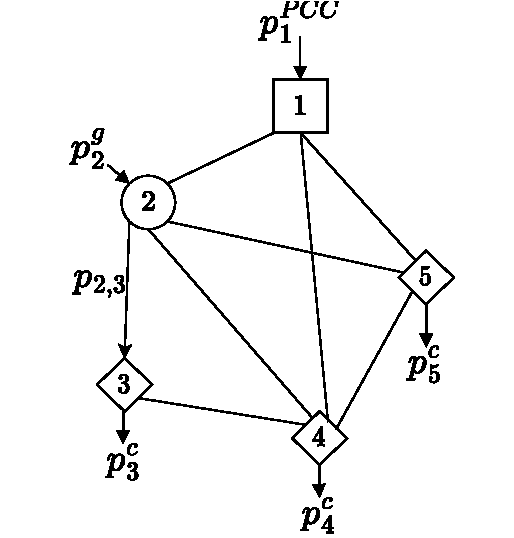
\includegraphics[width=\textwidth]{images/netwok_flow-Page-1_drawio.pdf}
\end{columns}
\end{frame}



\begin{frame}{A first basic generator model}
\begin{columns}
\column{0.65\linewidth}
    A generator is attached to a node $u$ and can output a power $p^g_u \geq 0$ $[MW]$ limited by a maximum power $\bar{P}^g_u$ $[MW]$. The associated production cost $[EUR/h]$ is $$c^g_{u,0} + c^g_{u,1}p^g_u.$$
\column{0.3\linewidth}
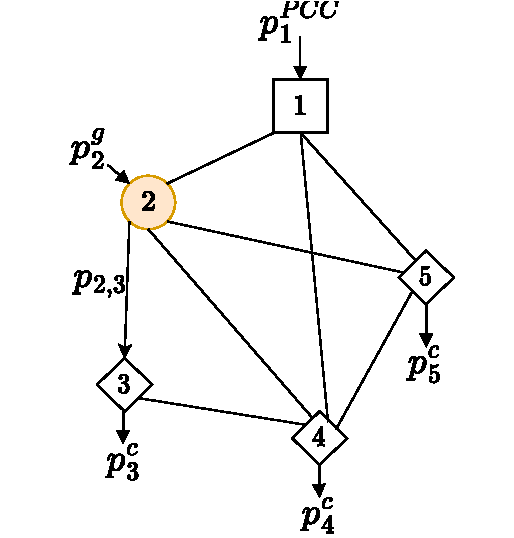
\includegraphics[width=\textwidth]{images/netwok_flow-Page-3_drawio.pdf}
\end{columns}
\end{frame}

\begin{frame}{Point of common coupling I}
\begin{columns}
\column{0.65\linewidth}
    The point of common coupling can be seen as a special generator that can either inject or consume power.
     Let 
    $$p^{PCC} = p^{PCC,+} - p^{PCC,-} \quad [MW] $$
    be the power injected by the PCC in the microgrid, with $p^{PCC,+} \geq 0$ and $p^{PCC,-} >= 0$.
    When it consumes power ($p^{PCC}\leq 0$), it means that the power generated in the microgrid exceeds the consumption and is thus pushed into the public grid.

\column{0.3\linewidth}
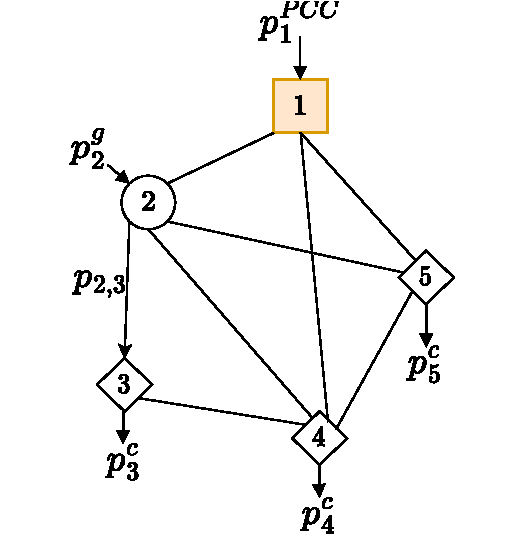
\includegraphics[width=\textwidth]{images/netwok_flow-Page-2_drawio.pdf}
\end{columns}
\end{frame}

\begin{frame}{Point of common coupling II}
\begin{columns}
\column{0.65\linewidth}
    The power exchanged with the public grid is limited, either physically or contractually, to $\bar{P}^{PCC}$: $$ -\bar{P}^{PCC} \leq p^{PCC} \leq \bar{P}^{PCC} \quad [MW].$$
    
    There is a cost $c^{PCC,+}$ $[EUR/MWh]$ associated with energy bought from the public grid and a revenue $c^{PCC,-}$ $[EUR/MWh]$ associated with energy injected into the public grid. We have $$c^{PCC,+} > c^{PCC,-}.$$
\column{0.3\linewidth}
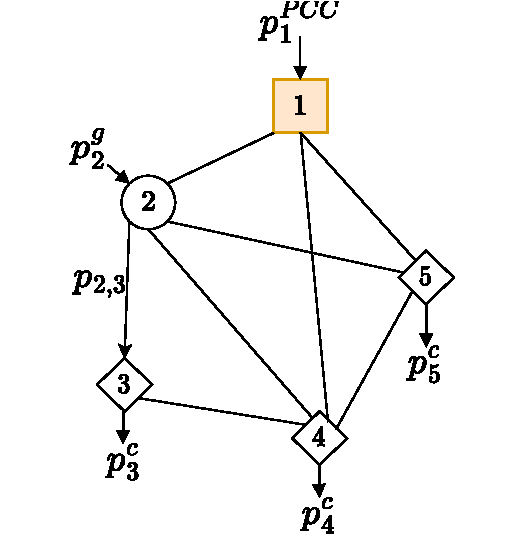
\includegraphics[width=\textwidth]{images/netwok_flow-Page-2_drawio.pdf}
\end{columns}
\end{frame}


\begin{frame}{Consumption nodes}
\begin{columns}
\column{0.65\linewidth}
    A load is attached to a consumption node $u$ and consumes a power $p^c_u \geq 0$ that cannot be modified.
\column{0.3\linewidth}
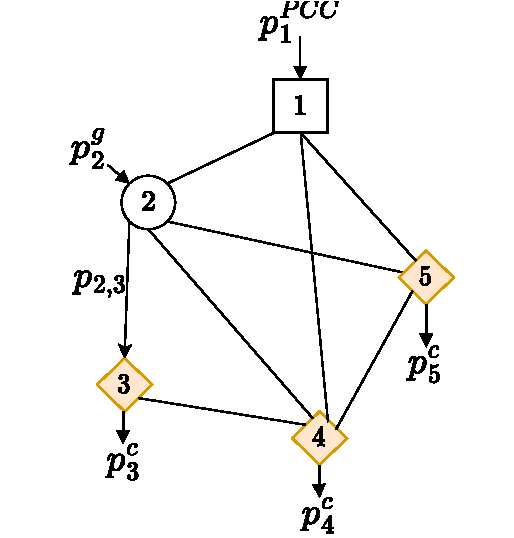
\includegraphics[width=\textwidth]{images/netwok_flow-Page-5_drawio.pdf}
\end{columns}
\end{frame}

\begin{frame}{Edges}
\begin{columns}
\column{0.65\linewidth}
An edge $(u,v)$ allows sending power $p_{u,v}$ from node $u$ to node $v$.
However, it has a maximum capacity $\bar{P}_{u,v}$ $[MW]$: 
$$-\bar{P}_{u,v}\leq p_{u,v} \leq \bar{P}_{u,v}.$$
\column{0.3\linewidth}
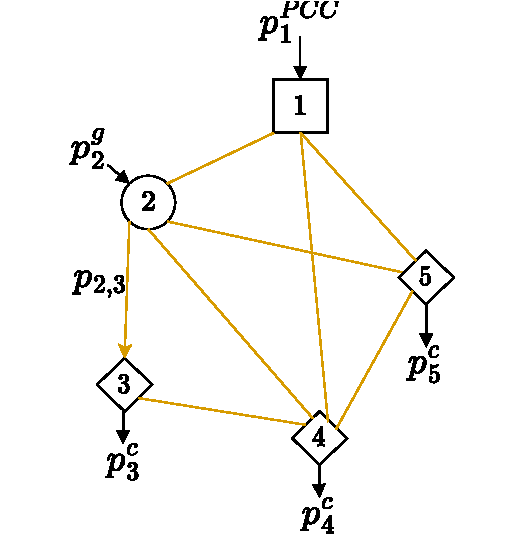
\includegraphics[width=\textwidth]{images/netwok_flow-Page-6_drawio.pdf}
\end{columns}
\end{frame}

\begin{frame}{Objective}

We aim to minimize the total cost of satisfying the demand while satisfying the constraints of the generators, PCC, edges, and the power balance at each node. 
    
\end{frame}

\begin{frame}{Formulate this problem as a linear program and solve it!}

\begin{itemize}
    \item A \alert{\href{https://colab.research.google.com/drive/1lrWL7sOrazTzlapVxcxrv_ZvVUZADC0h?usp=sharing}{template Google Colab is available here}}
    \item It uses 
    \begin{itemize}
        \item Python as a general programming language
        \item Pyomo as mathematical programming modeling library for Python
        \item Ipopt as a solver, which receives the problem from Pyomo and returns a solution, if any.
    \end{itemize}
    \item More instruction in the Colab template.
\end{itemize}
\end{frame}
